\documentclass[12pt]{article}
\usepackage[a4paper, margin=0.75in]{geometry}
\usepackage[document]{ragged2e}
\usepackage{graphicx}
\usepackage{multicol}
\graphicspath{ {./images/} }
\usepackage{enumerate}
\usepackage{framed}
\usepackage{amsmath,amsfonts,amsthm,thmtools,amssymb,mathtools,commath}
\usepackage{physics}
\usepackage{tikz}
\usetikzlibrary{mindmap}
\usepackage{caption}
\usepackage{xcolor}
\usepackage[most]{tcolorbox}
\usepackage{cleveref}


%%%%%%%%%%%%%%%%
%  Definition  %
%%%%%%%%%%%%%%%%
\tcbuselibrary{theorems,skins,hooks}
\newtcbtheorem[number within=subsection]{definition}{Definition}%
{
    % theorem style=definition,
    enhanced,
	before skip=2mm,after skip=2mm, colback=cyan!5,colframe=cyan!80!black,boxrule=0.5mm,
	attach boxed title to top left={xshift=1cm,yshift*=1mm-\tcboxedtitleheight},
	boxed title style={frame code={
					\path[fill=cyan]
					([yshift=-1mm,xshift=-1mm]frame.north west)
					arc[start angle=0,end angle=180,radius=1mm]
					([yshift=-1mm,xshift=1mm]frame.north east)
					arc[start angle=180,end angle=0,radius=1mm];
					\path[left color=cyan!30!black,right color=cyan!30!black,
						middle color=cyan!50!black]
					([xshift=-2mm]frame.north west) -- ([xshift=2mm]frame.north east)
					[rounded corners=1mm]-- ([xshift=1mm,yshift=-1mm]frame.north east)
					-- (frame.south east) -- (frame.south west)
					-- ([xshift=-1mm,yshift=-1mm]frame.north west)
					[sharp corners]-- cycle;
				},interior engine=empty,
		},
	fonttitle=\bfseries,
	title={#2},#1
}{def}


%%%%%%%%%%%%%
%  Theorem  %
%%%%%%%%%%%%%
\tcbuselibrary{theorems,skins,hooks}
\newtcbtheorem[use counter from=definition]{theorem}{Theorem}%
{
    theorem style=plain,
    enhanced,
    colframe=green,
    boxrule=1pt,
    titlerule=0mm,
    toptitle=1mm,
    bottomtitle=1mm,
    fonttitle=\bfseries,
    fontupper=\mdseries\itshape,
    coltitle=green!30!black,
    colbacktitle=cyan!15!white,
    colback=green!10,
    description font=\bfseries\sffamily
}{thrm}


%%%%%%%%%%%%%%
% Corollary  %
%%%%%%%%%%%%%%
 \tcbuselibrary{theorems,skins}
 \newtcbtheorem[use counter from=theorem]{corollary}{Corollary}%
 {
    theorem style=plain,
    enhanced,
    colframe=green,
    frame hidden,
    titlerule=0mm,
    toptitle=1mm,
    bottomtitle=1mm,
    fonttitle=\bfseries,
    fontupper=\mdseries\itshape,
    coltitle=green!30!black,
    colbacktitle=cyan!15!white,
    colback=green!10,
    description font=\bfseries\sffamily
 }{corl}


%%%%%%%%%%%%%
%  Example  %
%%%%%%%%%%%%%
\tcbuselibrary{theorems,skins,hooks}
\newtcbtheorem[number within=section]{example}{Example}%
{
	enhanced,
	breakable,
	colback = gray!5,
	frame hidden,
	boxrule = 0sp,
	borderline west = {2pt}{0pt}{gray},
	sharp corners,
	detach title,
	before upper = \tcbtitle\par\smallskip,
    coltitle=gray!70!black,
	fonttitle = \bfseries\sffamily,
	description font = \mdseries\bfseries
}
{xmp}


%%%%%%%%%%%%%%
%  Exercise  %
%%%%%%%%%%%%%%
\tcbuselibrary{theorems,skins,hooks}
\newtcbtheorem[number within=section]{exercise}{Exercise}%
{
    enhanced,
    breakable,
    colback=black!5,
    colframe=black!30,
    left=0.5em,
    before skip=10pt,
    after skip=10pt,
    boxrule=0pt,
    boxsep=0pt,
    arc=0pt,
    outer arc=0pt,
    borderline west={3pt}{0pt}{black!30},
}{exc}

%%%%%%%%%%
%  Note  %
%%%%%%%%%%
\usetikzlibrary{arrows,calc,shadows.blur}
\tcbuselibrary{skins}
\newtcolorbox{note}[1][]{%
	enhanced jigsaw,
	colback=gray!20!white,%
	colframe=gray!80!black,
	size=small,
	boxrule=1pt,
	title=\textbf{Note:-},
	halign title=flush center,
	coltitle=black,
	breakable,
	drop shadow=black!50!white,
	attach boxed title to top left={xshift=1cm,yshift=-\tcboxedtitleheight/2,yshifttext=-\tcboxedtitleheight/2},
	minipage boxed title=1.5cm,
	boxed title style={%
			colback=white,
			size=fbox,
			boxrule=1pt,
			boxsep=2pt,
			underlay={%
					\coordinate (dotA) at ($(interior.west) + (-0.5pt,0)$);
					\coordinate (dotB) at ($(interior.east) + (0.5pt,0)$);
					\begin{scope}
						\clip (interior.north west) rectangle ([xshift=3ex]interior.east);
						\filldraw [white, blur shadow={shadow opacity=60, shadow yshift=-.75ex}, rounded corners=2pt] (interior.north west) rectangle (interior.south east);
					\end{scope}
					\begin{scope}[gray!80!black]
						\fill (dotA) circle (2pt);
						\fill (dotB) circle (2pt);
					\end{scope}
				},
		},
	#1,
}


\title{
    \textbf{Experiment 9} \\
    \textbf{Frequency Response of Low Pass Filter}
}

\author{
    Turja Roy \\
    ID: 2108052
}
\date{}

\begin{document}
\maketitle

\section{Objective}
\begin{enumerate}
    \item To determine the low pass filter frequency response of an RC circuit.
    \item To measure the cut off frequency and observe the attenuation rate.
    \item To compare the graph of simulation data and practical data.
\end{enumerate}

\section{Apparatus}
\begin{multicols}{2}
    \begin{enumerate}
        \item Resistors
        \item Capacitors
        \item Oscilloscope
        \item Breadboard
    \end{enumerate}
    \columnbreak
    \begin{enumerate}
        \item Wires
        \item Function Generator
        \item DC Power Supply
        \item Multimeter
    \end{enumerate}
\end{multicols}

\section{Circuit Diagram}
\begin{figure}[h]
    \centering
    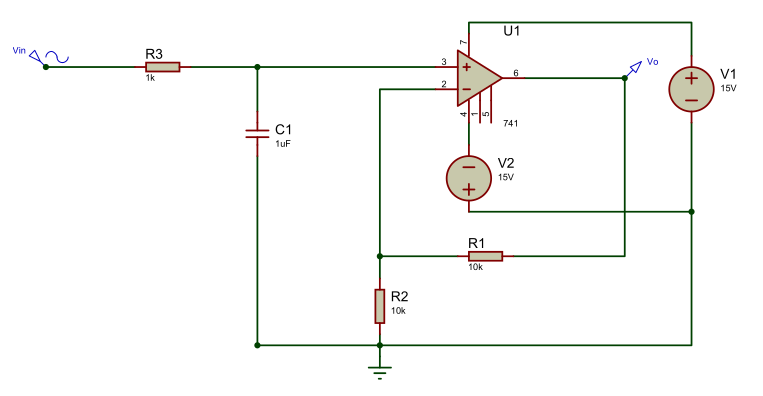
\includegraphics[width=0.8\textwidth]{LPF.png}
    \caption{Low Pass Filter Circuit}
\end{figure}

\section{Result Analysis}

\subsection{Data Table}
The low pass RC circuit allows low-frequency signals to pass while attenuating high-frequency signals. The detailed data is shown in Table 1. The cutoff frequency is observed at the point where the output voltage drops to 70.7\% of the input voltage. The attenuation rate is -20dB/decade beyond the cutoff frequency

\begin{table}[h!]
    \centering
    \caption{Practical and Simulated Data of Low Pass Filter}
    \begin{tabular}{rrrr}
        \hline
        Vin (V) &  Frequency (Hz) &  Practical Data Av (dB) &  Simulated Data Av (dB) \\
        \hline
        1 &             0.1 &                 4.959465 &                 4.959465 \\
        1 &             1.0 &                 5.249022 &                 4.959465 \\
        1 &             1.5 &                 5.057061 &                 4.860761 \\
        1 &             2.0 &                 5.343435 &                 4.810985 \\
        1 &             2.5 &                 5.436832 &                 4.959465 \\
        1 &             3.0 &                 5.620667 &                 4.910253 \\
        1 &             3.5 &                 5.666025 &                 5.057061 \\
        1 &             4.0 &                 6.277344 &                 5.153571 \\
        1 &             4.5 &                 6.648769 &                 5.249022 \\
        1 &             5.0 &                 6.808882 &                 5.249022 \\
        1 &             5.5 &                 7.158697 &                 5.296356 \\
        1 &             6.0 &                 7.421357 &                 5.483157 \\
        1 &             7.0 &                 7.889034 &                 5.620667 \\
        1 &             8.0 &                 8.198662 &                 5.666025 \\
        1 &            10.0 &                 6.107027 &                 5.800692 \\
        1 &            50.0 &                 6.887845 &                 5.845121 \\
        1 &           100.0 &                 7.004960 &                 5.933304 \\
        1 &           110.0 &                 7.272240 &                 5.977062 \\
        1 &           150.0 &                 6.769130 &                 6.063921 \\
        1 &           200.0 &                 5.390259 &                 6.063921 \\
        1 &           250.0 &                 4.243752 &                 6.149921 \\
        1 &           300.0 &                 3.167250 &                 6.235077 \\
        1 &           350.0 &                 2.076074 &                 6.063921 \\
        1 &           400.0 &                 1.437640 &                 0.827854 \\
        1 &           450.0 &                 0.668475 &                 0.984360 \\
        1 &           500.0 &                 0.086427 &                 0.086427 \\
        1 &           600.0 &                -1.012200 &                -1.411621 \\
        1 &           700.0 &                -1.830300 &                -1.514414 \\
        1 &           900.0 &                -3.223018 &                -3.609121 \\
        1 &          1000.0 &                -3.876401 &                -3.741733 \\
        1 &          1500.0 &                -5.848596 &                -4.582960 \\
        1 &          2000.0 &                -7.130946 &                -6.375175 \\
        1 &          3000.0 &                -8.404328 &                -7.744323 \\
        1 &          4000.0 &                -9.118639 &                -8.873950 \\
        1 &          5000.0 &                -9.370422 &                -9.118639 \\
        1 &         10000.0 &                -9.118639 &                -9.118639 \\
        1 &         50000.0 &                -9.370422 &                -9.118639 \\
        \hline
    \end{tabular}
\end{table}

\newpage
\subsection{Graph}

\begin{figure}[h]
    \centering
    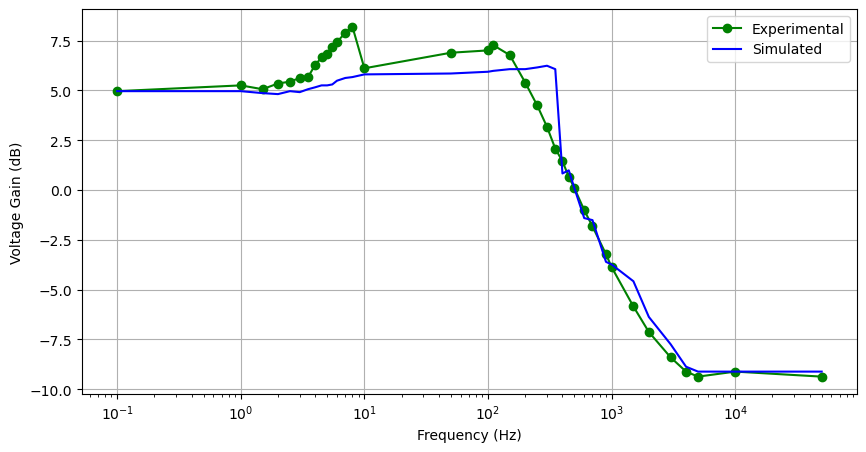
\includegraphics[width=0.8\textwidth]{LPF_Graph.png}
    \caption{Frequency Response of Low Pass Filter}
\end{figure}

In this graph, the x-axis represents the frequency in Hz and the y-axis represents the gain in dB. The graph shows that the low pass filter blocks the lower frequency and passes the higher frequency. The cutoff frequency is observed at 500Hz where the output voltage drops to 70.7\% of the input voltage. The attenuation rate is -20dB/decade beyond the cutoff frequency.

\section{Discussion}

The low pass filter is a circuit that allows low-frequency signals to pass while attenuating high-frequency signals. The cutoff frequency is the point where the output voltage drops to 70.7\% of the input voltage. The attenuation rate is -20dB/decade beyond the cutoff frequency. The practical and simulated data of the low pass filter are shown in Table 1. The graph of the frequency response of the low pass filter is shown in Figure 1. The graph shows that the low pass filter blocks the lower frequency and passes the higher frequency.

\end{document}

